\clearpage
\newpage

\section[Тестирование]{\large \centering Тестирование}
\hspace{\parindent} Для всесторонней оценки работы программы результат выравнивания и производительность сравнивали с единственным существующим ее аналогом --- MACSE (пункт~\ref{MACSE}), который является признанным программным решением. 

\subsection[Оценка качества выравнивания]{\large Оценка качества выравнивания}
\hspace{\parindent} В качестве тестовых задач для оценки получаемых выравниваний использовали наборы последовательностей, которые применяли авторы MACSE в работе~\cite{MACSE}. Для каждой тестовой задачи из набора строили множественные выравнивания с помощью программ MACSE и multy. Полученные результаты попарно сравнивались функцией оценки (листинг~\ref{lst:marker}). Идея метода заключена в сопоставлении выравненных блоков последовательностей сравниваемых результатов и вычислении среднего арифметического долей совпадений в каждом из выравниваний:
\begin{equation*}
\dfrac{\dfrac{count}{len(P_1)} + \dfrac{count}{len(P_2)}}{2}
\end{equation*}
где $count$ --- число совпадений, а $len(P_i)$ --- длина $i$-го выравнивания. Совпадением считается сопоставление одинаковых нуклеотидов или аминокислот, лишние разрывы пропускаются до следующего символа. Алгоритм оценки реализован на языке программирования Python 2.7.8 (листинг~\ref{lst:marker}).
\begin{algorithm}
	\caption{Реализация алгоритма сравнения двух выравниваний} \label{lst:marker}
	\begin{lstlisting}
score = 0.
while index1 < len(seq1) and index2 < len(seq2):
    if (seq1[index1] == seq2[index2]):
      score += 1
      index1 += 1
      index2 += 1
    else:
      if (seq1[index1] == '-'):
        index1 += 1
      else:
        if (seq2[index2] == '-'):
	\end{lstlisting}
\end{algorithm}

\begin{algorithm}
	\begin{lstlisting}
          index2 += 1      
        else:
          index1 += 1
          index2 += 1
total += (score / len(seq1) + score / len(seq2)) / 2.
	\end{lstlisting}
\end{algorithm}
Здесь $seq1$ и $seq2$ сравниваемые последовательности, а $total$ --- оценка похожести выравниваний. При сравнении множественных выравниваний вычисляется среднее арифметическое полученных парных оценок.\\
\indent В качестве исходных данных для тестирования был взят проверенный тестовый набор последовательностей MACSE. В связи с тем, что решение MACSE строит выравнивание с использованием дополнительных функций обновления и улучшения результатов при выравнивании псевдогенов и не имеет возможности их отключения, некоторые тесты были пропущены. \\
\indent Обоим программам на вход подавались одинаковые параметры выравнивания. Согласно нашей функции оценки мы получили среднее значение совпадений 90,5\% на нуклеотидном и 92,1\% на аминокислотном уровне. Наличие различий в выдаваемых выравниваний естественно, так как алгоритмы имеют общую идею, но совершенно разную реализацию. В разработанном решении используются две матрицы замен: для нуклеотидного и аминокислотного уровней, в отличие от решения MACSE, ограничивающегося только оценкой уровня аминокислот. Более высокое качество выравнивания на аминокислотном уровне доказывает правильность работы созданного алгоритма. Полученные результаты являются удовлетворительными.\\
\indent На рисунках \ref{ris:MM_AA} и \ref{ris:MM_NT} показаны построенные выравнивания для одного из блоков тестов MACSE. Представлены только различающиеся участки полученных выравниваний. Общая длина на нуклеотидном уровне --- 426 остатков.

\begin{figure}[H]
	\center{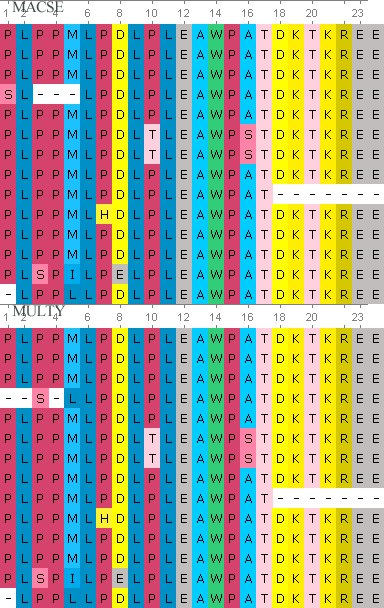
\includegraphics[width=0.9\linewidth]{aaTest}}
	\caption{Сравнение множественных выравниваний последовательностей аминокислот}
	\label{ris:MM_AA}
\end{figure}

\begin{figure}[H]
	\center{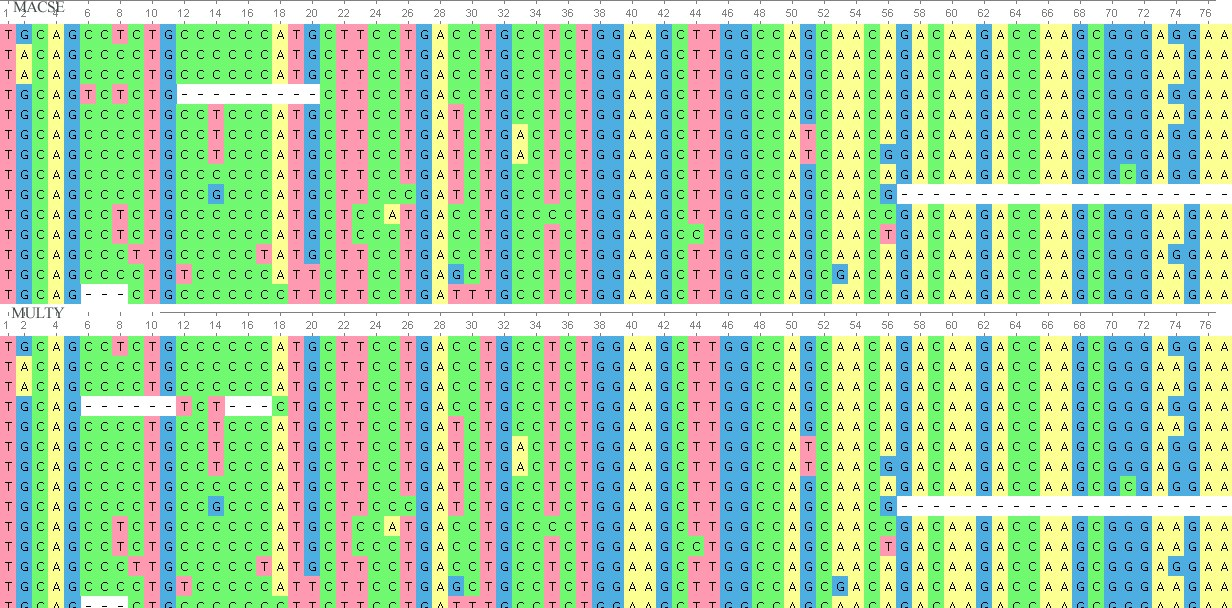
\includegraphics[width=1\linewidth]{NTtest}}
	\caption{Сравнение множественных выравниваний последовательностей нуклеотидов}
	\label{ris:MM_NT}
\end{figure}

	

\subsection[Оценка производительности]{\large Оценка производительности}
\hspace{\parindent} Производительность разработанного алгоритма против существующей программы парного выравнивания MACSE оценивалась на группах синтетических тестов --- наборы созданных случайных последовательностей нуклеотидов заданной длины (на листинге~\ref{lst:testcreater} представлен код программы генерации тестовых данных).  Тестирование происходило на машине с двумя шестиядерными процессорами Intel Xeon E5645 под управлением ОС Linux Debian 7 (wheezy) и объемом оперативной памяти 24 ГБ. Результаты тестирования представлены в таблице и на гистограмме (рисунок~\ref{ris:gist}).
\begin{algorithm}[H]
	\caption{Реализованные на Python 2.7.8 функции создания набора тестовых данных} \label{lst:testcreater}
	\begin{lstlisting}
import random, string

def CreateSeq(length = 1000):
    return ''.join(random.choice("ACGT") \
    		for _ in range(length))

def CreateData(seq_count, seq_length):
    data=[]
	\end{lstlisting}
\end{algorithm}

\begin{algorithm}
	\begin{lstlisting}
    for i in range(seq_count):
        data.append(">seq"+str(i))
        data.append(CreateSeq(seq_length))
    return data
	\end{lstlisting}
\end{algorithm}

Из графиков и таблицы хорошо видно серьезное замедление времени выполнения на больших тестах для обоих алгоритмов (рисунок~\ref{ris:multyvsMACSE}). При тестировании было рассмотрено несколько сборок разработанной программы: используя компилятор gcc версии 4.8.4 с флагом -O3 и компилятор intel icpc версии 15.0.3 с различными флагами оптимизации. Одна из выбранных опций: -fast, которая включает в себя следующие ключи icpc:
\begin{equation*}
\texttt{-xHOST -O3 -ipo -no-prec-div -static -fp-model fast=2}
\end{equation*}

\begin{figure}[h]
	\begin{minipage}[h]{0.49\linewidth}
		\center{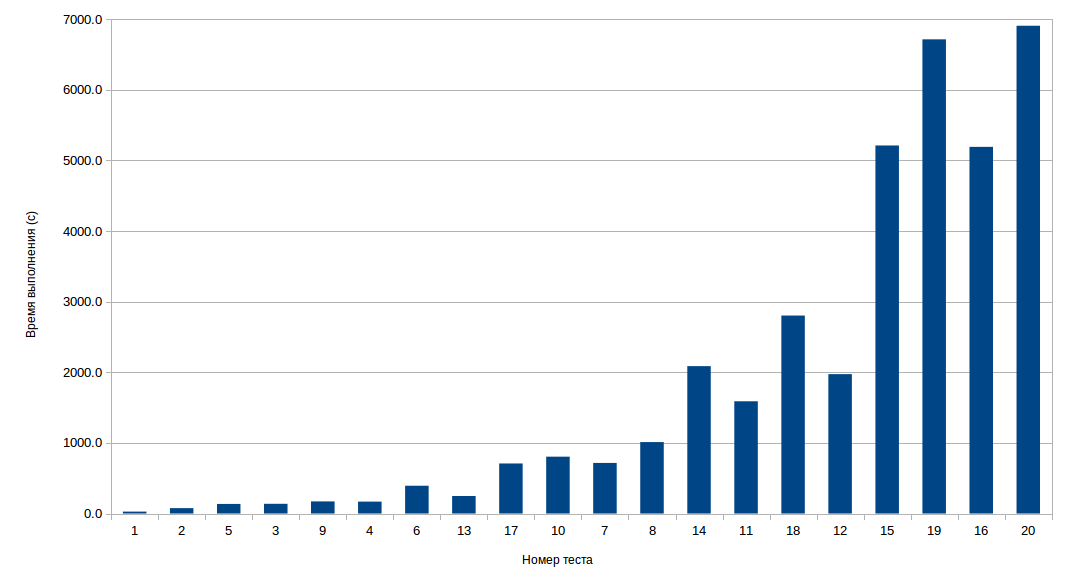
\includegraphics[width=1\linewidth]{MACSEtest} \\ а) MACSE}
	\end{minipage}
	\hfill
	\begin{minipage}[h]{0.49\linewidth}
		\center{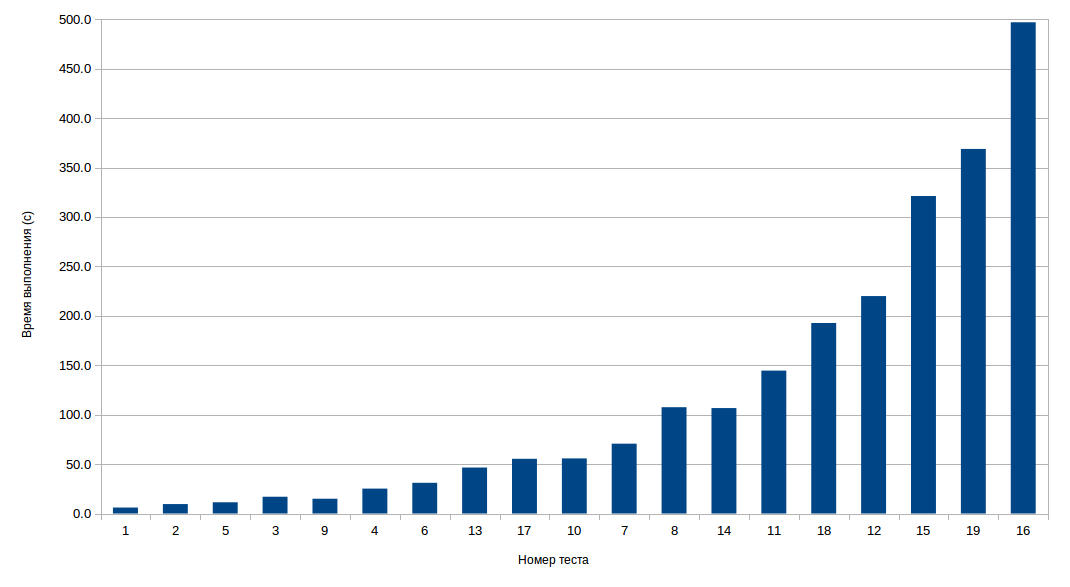
\includegraphics[width=1\linewidth]{multytest} \\ б) multy}
	\end{minipage}
	\caption{График роста времени выполнения при увеличении объема входных данных}
	\label{ris:multyvsMACSE}
\end{figure}

Также, компилятор intel предоставляет возможность скомпилировать пробную версию программы, запустить ее на заданном наборе тестов и по результатам выполнения произвести повторную сборку, что потенциально может дать прирост скорости. Для этого необходимо воспользоваться опцией -prof-gen:
\begin{equation*}
\texttt{-O3 -no-prec-div -fp-model fast=2 -xHost -prof-gen}
\end{equation*}
После компиляции производится запуск программы на тестовом наборе данных для генерации профилей производительности *.dyn и *.dpi, а затем выполняется повторная сборка. Аналогичным образом используется ключ автоматической параллелизации -parallel:
\begin{equation*}
\texttt{-O3 -no-prec-div -fp-model fast=2 -xHost -prof-gen -parallel}
\end{equation*}  

\begin{landscape}
\begin{figure}[h]
	\center{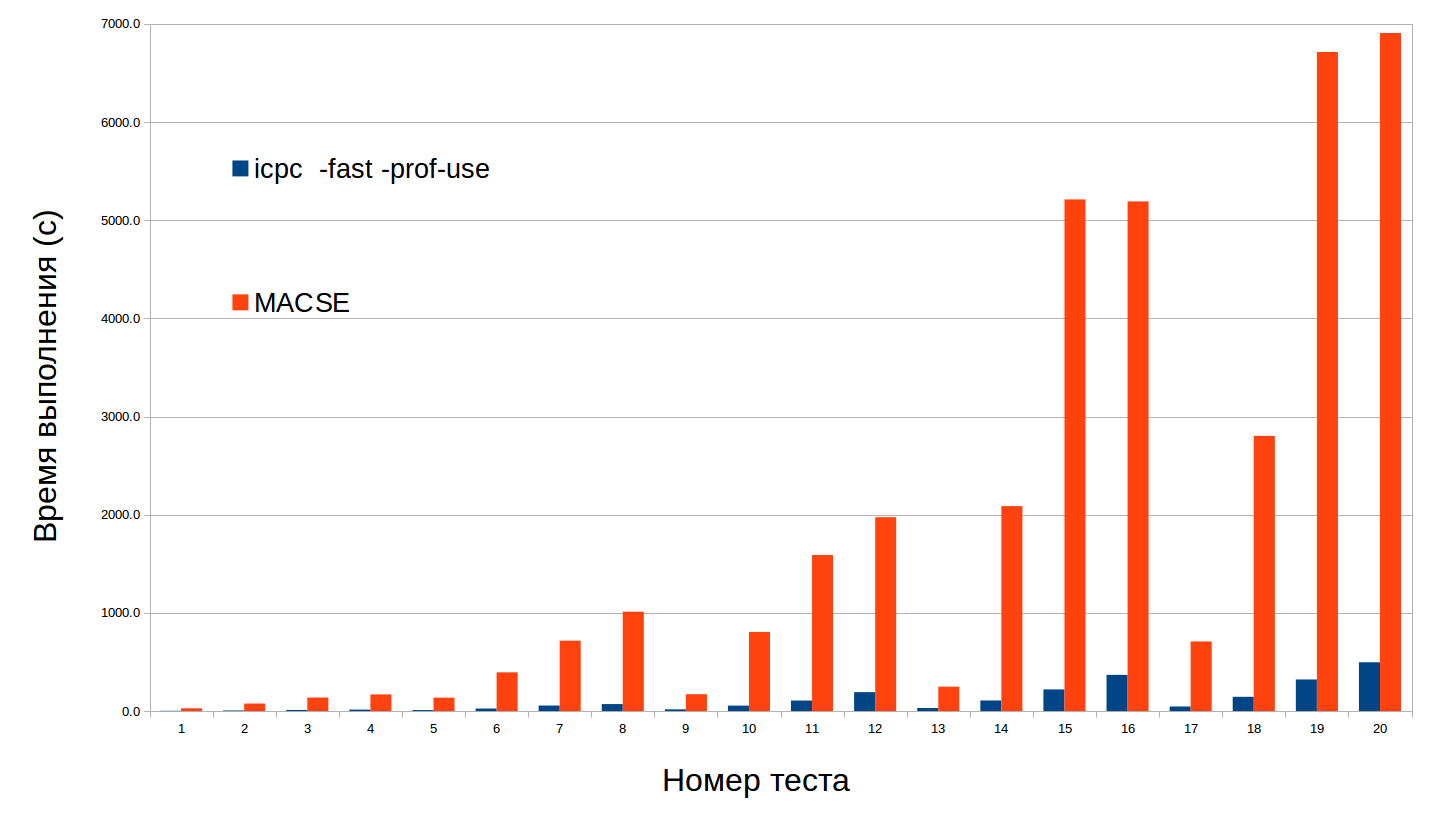
\includegraphics[width=1.\linewidth]{gist.png}}
	\caption{Время выполнения тестов разработанного алгоритма и MACSE}
	\label{ris:gist}
\end{figure}
\end{landscape}

\begin{landscape}
\begin{table}[htbp]
\small
\caption{Результаты тестирования}
\begin{flushright}
\begin{longtable}{|p{1cm}|*{2}{p{3cm}|}*{2}{p{1.8cm}|}*{3}{p{2.8cm}|}*{2}{p{1.8cm}|}}
\hline
\multicolumn{ 1}{|p{1cm}|}{Номер теста} & \multicolumn{ 1}{p{3cm}|}{Длина поледовательностей} & \multicolumn{ 1}{p{3cm}|}{Количество последовательностей} & \multicolumn{ 7}{p{15.6cm}|}{Время выполнения (с)} \\ \cline{ 4- 10}
\multicolumn{ 1}{|p{1cm}|}{} & \multicolumn{ 1}{p{3cm}|}{} & \multicolumn{ 1}{p{3cm}|}{} & \multicolumn{ 6}{p{10.8cm}|}{Опции компиляции } & \multicolumn{ 1}{p{1.8cm}|}{MACSE} \\ \cline{ 4- 9}
\multicolumn{ 1}{|p{1cm}|}{} & \multicolumn{ 1}{|p{3cm}|}{} & \multicolumn{ 1}{p{3cm}|}{} & \multicolumn{1}{p{1.8cm}|}{icpc -O0} & \multicolumn{ 1}{p{1.8cm}|}{icpc -fast} & \multicolumn{1}{p{1.8cm}|}{icpc  -fast -prof-use} & \multicolumn{1}{p{1.8cm}|}{icpc -fast -parallel} & \multicolumn{ 1}{p{1.8cm}|}{icpc -fast -prof-use -parallel} & \multicolumn{1}{p{1.8cm}|}{gcc -O3} & \multicolumn{ 1}{p{1.8cm}|}{} \\ 
\hline
1 & 500 & 5 & 11,9 & 2,4 & 2,3 & 2,3 & 2,2 & 2,8 & 27,3 \\ \hline
2 & 500 & 10 & 40,2 & 6,7 & 6,1 & 7,2 & 6,1 & 7,7 & 76,3 \\ \hline
3 & 500 & 15 & 76,0 & 12,5 & 11,4 & 12,0 & 11,1 & 14,0 & 137,8 \\ \hline
4 & 500 & 20 & 115,0 & 18,7 & 15,0 & 16,0 & 15,7 & 18,5 & 169,3 \\ \hline
5 & 1000 & 5 & 48,8 & 9,1 & 9,6 & 8,8 & 8,1 & 10,8 & 136,3 \\ \hline
6 & 1000 & 10 & 165,3 & 27,4 & 25,2 & 28,5 & 25,3 & 34,7 & 394,3 \\ \hline
7 & 1000 & 15 & 396,3 & 62,4 & 55,8 & 62,9 & 60,9 & 69,9 & 716,9 \\ \hline
8 & 1000 & 20 & 556,7 & 75,1 & 70,7 & 86,7 & 74,8 & 87,4 & 1012,1 \\ \hline
9 & 1500 & 5 & 100,5 & 18,1 & 17,0 & 18,1 & 16,6 & 22,0 & 171,6 \\ \hline
10 & 1500 & 10 & 384,5 & 60,4 & 55,4 & 65,2 & 57,0 & 78,1 & 805,8 \\ \hline
11 & 1500 & 15 & 830,0 & 117,5 & 106,7 & 115,6 & 106,0 & 136,0 & 1589,4 \\ \hline
12 & 1500 & 20 & 1551,4 & 205,2 & 192,7 & 203,8 & 196,3 & 252,4 & 1974,1 \\ \hline
13 & 2000 & 5 & 184,9 & 33,2 & 31,1 & 40,8 & 29,3 & 39,9 & 248,2 \\ \hline
14 & 2000 & 10 & 669,4 & 106,7 & 107,6 & 103,8 & 101,8 & 124,4 & 2087,5 \\ \hline
15 & 2000 & 15 & 1540,5 & 219,7 & 219,9 & 274,0 & 203,2 & 257,5 & 5212,5 \\ \hline
16 & 2000 & 20 & 2909,8 & 397,5 & 368,8 & 401,8 & 375,6 & 529,8 & 5191,9 \\ \hline
17 & 2500 & 5 & 290,3 & 53,4 & 46,5 & 50,9 & 46,2 & 62,1 & 708,8 \\ \hline
18 & 2500 & 10 & 1006,8 & 156,9 & 144,6 & 166,8 & 143,6 & 187,9 & 2803,2 \\ \hline
19 & 2500 & 15 & 2417,3 & 344,1 & 321,2 & 352,0 & 334,8 & 408,6 & 6714,3 \\ \hline
20 & 2500 & 20 & 3944,9 & 596,8 & 496,9 & 572,0 & 511,3 & 665,7 & 6907,3 \\ \hline
\end{longtable}
\end{flushright}
\label{tabular:results}
\end{table}
\end{landscape}